
\subsection{The Collapse}

\subsubsection{Fallback Logic, Live}


Nearly half the fund’s value was incinerated before lunch.

There was no headline. No flash alert.
Just a stillness that settled over the floor like static before a storm.

The espresso machine hissed. Someone coughed. Then nothing.
Slack channels slowed. No one dared tag the CIO.
Even the banter—the armor traders wore when red screens stacked—had vanished.

Screens flickered, paused, then froze.
Risk dashboards spit out nonsense.
Volatilities spiked off-chart. Some assets rendered as “NaN.”

From the corner row, Neha leaned forward, squinting at her terminal.
“IG credit’s gone no-bid,” she muttered. “I mean, literally. No. Bid.”

Two desks over, Leo didn’t look up.
“Try IG 3-5 year. Should show some depth.”

Neha scrolled. Her lips parted slightly.

“Eighty-eight last night,” she said quietly. “Seventy-four now. Wide as hell. And that’s from one guy in Zurich.”

She turned.

“That’s not a quote. That’s a cry for help.”

Across the floor, someone dropped a pen. It sounded loud.

A junior stood by the compliance wall monitor, pale.

“Uh,” he said, voice dry. “Collateral notice just hit. BNY. Seized the TRS sleeve.”

“Already?” Leo asked. “They called?”

The junior shook his head. “Auto-exec. Trigger clause. 20bps threshold breach.”

No one spoke. Then Neha again:

“Jesus. That’s deep in the annex.”

They all knew what that meant:
ISDA fallback logic. The kind no one ever expects to see run.
The kind no one even checks anymore.

And now it was live.

\medskip

\begin{TechnicalSidebar}{What’s in an ISDA Annex?}

  At first glance, an ISDA agreement looks like a partnership.

  \medskip
  
  But it isn’t.

  \medskip
  
  It’s a legal machine — and the annexes are where the machine learns how to bite.
  
  \medskip
  
  The \textbf{ISDA Master Agreement} is the boilerplate. It governs the relationship and defines the rules. But the real leverage lives in the attachments:

  \medskip
  
  \begin{itemize}
    \item \textbf{Schedule A}  
    Custom terms. This is where counterparties bury modifications, exceptions, and definitions that override the defaults. Want to enable collateral sweeps during market stress? You don’t change the master — you bury it in Schedule A, Paragraph 13.2(c).
  
    \item \textbf{Credit Support Annex (CSA)}  
    This governs margin. It spells out which assets count as collateral, how often they’re revalued, and how quickly they must be posted or returned. It also defines what happens when the market stops cooperating.
  
    \item \textbf{Definitions Booklets}  
    A running catalog of what technical terms mean (e.g., “Close-Out Amount,” “Eligible Collateral,” “Valuation Agent”). Updated over time. Seemingly trivial — until you realize that a clause like “reasonable discretion” can move \$100 million in five minutes.
  
    \item \textbf{Confirmations}  
    Trade-by-trade terms. These are the receipts — the specific transactions that inherit all the machinery above them.
  \end{itemize}
  
  \medskip
  
  The scary part?

  \medskip
  
  These annexes are rarely read in real time.  
  They’re agreed upon months (or years) before a crisis.  
  But once the thresholds are breached, they don’t ask. They execute.
  
\end{TechnicalSidebar}

\medskip

\subsubsection{Collateral Optimization}

The Bloomberg feed refreshed again—briefly—and then glitched.
A red square blinked, then vanished.

“Clearing bank just swept the Treasuries,” someone called out from middle office, breath short. “Repo desk’s confirming execution.”

“What size?” Neha asked, already knowing it would be bad.

“Four hundred twenty mil,” came the reply. “Dumped into the open. No ladder. No hedge.”

Leo didn’t look up. “That market’s a puddle right now. That’s not a sale. That’s a splash.”

At the far end of the floor, the legal pod was huddled over PDFs.

A junior scrolled furiously, finger tracing dense clauses. “Paragraph 13.2(c), Schedule A... says they can sweep the reserve account—”

“How much?” asked someone from Treasury.

“Ninety-two million,” the junior replied, still reading. “Labeled as ‘collateral optimization.’ No advance notice required.”

Someone cursed, softly but with precision.

“They’re not even pretending,” Neha said. “That’s not strategy anymore. That’s bloodflow.”

An associate from Legal—barely a year out of law school—asked it aloud:

“Can they do that?”

Compliance didn’t flinch. The director barely turned from her terminal.

“They already did,” she said. “And yes. The docs are clean. Everything’s trigger-based.”

She exhaled and tapped her screen. “These aren’t partners. They’re counterparties.”

Leo stood, slowly.

“Strategic assets,” he said. “That’s what we called them on the investor deck.”

Neha turned toward him, eyes hard.

“They’re not assets anymore,” she said. “They’re flags.”

And around them, the room held its silence. Not frozen. Not panicked. Just very, very still.

Because in a derivative stack, relationships don’t unwind.
They collapse.
And once the margin logic starts, it doesn’t ask for context.
It just clears the line.

\medskip

\begin{figure}[H]
  \centering
  \resizebox{\textwidth}{!}{ % ← scales TikZ to full page width
  \begin{tikzpicture}[
    node distance=0.7cm and 1.5cm,
    box/.style={draw, fill=gray!15, rounded corners, align=center, minimum width=4.5cm, minimum height=1cm},
    edge/.style={-latex, thick},
    label/.style={font=\small\itshape}
  ]

  % Top document
  \node[box, fill=gray!20] (master) {\textbf{ISDA Master Agreement}};

  % Schedule
  \node[box, below=of master] (schedule) {\textbf{Schedule A} \\ (Custom Terms \& Triggers)};
  \draw[edge] (master) -- (schedule);

  % CSA
  \node[box, below=of schedule] (csa) {\textbf{Credit Support Annex (CSA)} \\ Margin Terms, Collateral Types};
  \draw[edge] (schedule) -- (csa);

  % Margin call engine
  \node[box, below=of csa] (engine) {\textbf{Margin Engine} \\ Variation / Initial Margin \\ Real-Time Recalculation};
  \draw[edge] (csa) -- (engine);

  % Assets
  \node[box, below left=of engine, xshift=-0.5cm] (assets) {\textbf{Eligible Collateral} \\ Treasuries, Cash, Bonds};
  \draw[edge] (assets.east) -- (engine.west);

  % Automated triggers
  \node[box, below right=of engine, xshift=0.5cm] (auto) {\textbf{Auto-Triggers} \\ Sweep Clauses, Optimization};
  \draw[edge] (engine.east) -- (auto.west);

  % Final output: margin call
  \node[box, below=2cm of engine, fill=red!10] (margincall) {\textbf{Collateral Call Issued} \\ Assets Seized or Transferred};
  \draw[edge] (engine) -- (margincall);

  % Annotations
  \node[label, right=0.5cm of schedule] {Custom risk terms};
  \node[label, right=0.5cm of csa] {Defines margining rules};
  \node[label, below=0.5cm of assets] {What the fund thought was “strategic”};
  \node[label, below=0.5cm of auto] {Silent clauses that execute automatically};

  \end{tikzpicture}
  }
  \caption*{The ISDA Stack: A tower of obligations that doesn’t care about context — just numbers. When stress hits, it doesn't call. It executes.}
\end{figure}

\medskip

\subsubsection{The Waterfall Seized}

The repo desk lights had turned amber an hour ago.
Now, they were red.

"Haircuts just widened again," said Julia, eyes flicking between terminals. "Agency MBS went from two to eight."

"Eight?" Tom spun his chair halfway around. "That's a fire-sale number."

Julia didn’t look up. "It’s clearing logic. CDS spreads triggered a margin recalibration—hourly cycle just hit. The engine’s recalculating in real time now."

Farther down the desk, a senior repo analyst pulled off his headset.

"We just got pinged on tri-party," he said. "BAML’s line is under intraday review. They want fresh margin. Now."

"Against what?" asked the treasury ops lead. "We gave them AAA tranches. They don’t get cleaner than that."

"Apparently they do now," came the dry reply. "Two downgrades just hit the desk. Not rating agency — internal model. Real-time stress mapping."

A Slack alert pinged twice — low tone, urgent flag.

"Goldman’s triggering the collateral waterfall," Julia said, reading. "Cash swept. Next up: AAA CLOs."

Tom checked the waterfall model. “That’s not supposed to flip until next week.”

"Well," she said, deadpan. "Markets don’t run on our calendar."

Across the room, another alert lit up.

“Wait,” someone said, staring at their screen. “That can’t be right. We’re seeing offers on 2-years at six handles. SIX.”

“No bids?”

“None. And the tape’s dry.”

One screen over, another message popped up — flagged red.

“Convertibles are next,” said the repo lead. “One of the clearing partners just swept a full block of IG convertibles. No request. Just clause-based.”

Someone from compliance stepped into the pit.

“They’re not in breach,” she said, before anyone asked. “The clause kicked automatically when the CDS coverage ratio hit the stress floor.”

“Which floor?” someone muttered.

“The one we all pretended didn’t exist,” Julia answered. “Schedule D. Margin Tier IV.”

The last message came without sound — just a silent push alert:

EQUITY COLLATERAL BLOCK SOLD.
UNFILLED.

Tom stared at the screen. “Equity tail’s gone.”

“No liquidity?”

“No buyers,” Julia said. “Just void.”

She looked up. “That was the last buffer.”

Across the floor, you could feel it — not noise, but a kind of compression.
A vacuum around the lungs.

They had built a waterfall — precise, orderly, loss-aware.
But this wasn’t a waterfall.
It was a drain.

And once it opened,
it didn’t ask.
It just seized.

\medskip

\begin{TechnicalSidebar}{How Funds Bleed}

  Margin calls don’t ask what’s strategic.  
  They take what’s liquid.
  
  \medskip
  
  When a fund enters a margin spiral, the liquidation follows a hierarchy: one that was agreed upon long before anyone 
  thought about stress-testing it.

  \medskip
  
  \begin{itemize}
    \item \textbf{Step 1: Cash Reserves}  
    The easiest to seize. Instant liquidity. Usually swept automatically by clearing brokers or counterparties.
    
    \item \textbf{Step 2: Government Bonds}  
    Often pledged in repo or as margin collateral. Treasuries are the first high-value assets to go. They’re also the least disruptive to sell—until they aren’t.
    
    \item \textbf{Step 3: High-Grade Credit}  
    AAA CLOs, IG corporate bonds, and short-dated paper. Technically “safe,” but vulnerable to sharp mark-to-market drops in a panic.
    
    \item \textbf{Step 4: Convertibles and Structured Products}  
    These sit in the grey zone—part bond, part equity. Illiquidity premiums spike when volatility rises. Haircuts widen quickly.
    
    \item \textbf{Step 5: Equities and Residuals}  
    The riskiest, most volatile assets. Often meant to provide upside, but dumped at fire-sale prices once everything else has been exhausted.
  \end{itemize}
  
  \medskip
  
  The irony?  
  By the time a fund is selling its growth bets, it’s already dead.  
  The bleeding starts at the top, with the assets everyone thinks are “safe.”

  \medskip
  
  That’s not a glitch.  
  That’s how the system was designed.
  
\end{TechnicalSidebar}

\medskip

\subsubsection{The Clause That Executed Itself}

The fluorescent hum above the trading pit had become audible — not because it grew louder, but because everything else had gone quiet.

\textit{Ping. Ping.}
Two Slack notifications from the prime brokerage desk.
Then nothing.

“Prime’s not responding,” said Kayla, headset off now, just staring at the blinking cursor. “They pinged. Then disappeared.”

“Disappeared how?” asked Raj from legal. “Disconnected?”

“No,” she said. “Protocol-dark. Margin-trigger clause just flipped. We’re past the call window.”

Tom frowned. “Already? We haven’t even—”

“Doesn’t matter.” Kayla cut him off. “We're inside the document now.”

A junior ops analyst stood up two rows back, holding a printed copy of the ISDA annex.

“I think we’re in Schedule F territory,” she said, thumbing through the stack. “Paragraph 10.4(a)(ii) — collateral seizure without counterparty consent in the event of cascading valuation triggers.”

Raj didn’t blink. “Yeah. That’s the one where we lose voice rights.”

“Voice rights?” asked Tom.

“You can’t even call to negotiate,” Raj said. “The clause handles itself.”

Another ping.
Then three terminals flashed red across the floor.

“More rebalancing orders just hit the wire,” said Julia. “Not from us — from the algorithms clearing downstream stress.”

“You mean their algorithms,” Tom clarified.

She nodded. “Yeah. We’re not driving this anymore.”

David watched from the end of the row, arms folded, unreadable.

Technically, the fund still existed.
Legally, it still had assets.
But control had passed — not to people, but to protocol.

Every valuation shock triggered margin.
Every margin call triggered rebalancing.
Every rebalance triggered liquidation.

And none of it required a human to say yes.

\textit{That part was already signed.}

“You ever seen this before?” Julia asked, voice flat.

“No,” said Tom. “But I’ve read about it.”

He paused.

“It’s like watching your own paperwork liquidate you.”

\medskip

\begin{figure}[H]
  \centering

  % === First row ===
  \begin{subfigure}[t]{0.45\textwidth}
  \centering
  \begin{tikzpicture}
    \comicpanel{0}{0}
      {Risk Officer}
      {Fund Controller}
      {Start with the reserves. Sweep the cash.}
      {(-0.6,-0.6)}
  \end{tikzpicture}
  \caption*{Step 1: Cash — instant, painless, and already gone.}
  \end{subfigure}
  \hfill
  \begin{subfigure}[t]{0.45\textwidth}
  \centering
  \begin{tikzpicture}
    \comicpanel{0}{0}
      {Fund Controller}
      {Repo Desk}
      {Next up — the Treasuries. Haircuts widened overnight.}
      {(0.6,-0.6)}
  \end{tikzpicture}
  \caption*{Step 2: Treasuries — liquid, safe, and first to bleed.}
  \end{subfigure}

  \vspace{1em}

  % === Second row ===
  \begin{subfigure}[t]{0.45\textwidth}
  \centering
  \begin{tikzpicture}
    \comicpanel{0}{0}
      {Repo Desk}
      {CIO}
      {We’re into AAA CLOs and IG credit. Haircuts just doubled.}
      {(-0.6,-0.6)}
  \end{tikzpicture}
  \caption*{Step 3: High-grade credit — safe on paper, shaky in panic.}
  \end{subfigure}
  \hfill
  \begin{subfigure}[t]{0.45\textwidth}
  \centering
  \begin{tikzpicture}
    \comicpanel{0}{0}
      {CIO}
      {Execution Desk}
      {Last line — the equity tail. Push what’s still bid.}
      {(0.6,-0.6)}
  \end{tikzpicture}
  \caption*{Step 4: Equities — dumped last, priced worst.}
  \end{subfigure}

  \caption*{Liquidation isn’t discretionary. It’s ranked. In stress, the system takes what’s easiest — and leaves you with what no one wants.}
\end{figure}

\medskip


\subsubsection{The Fire Sale Begins}

The room smelled like burnt coffee and printer toner.

By Friday morning, the eleventh floor war room was full — Gantt charts on one wall, redemption notices printing nonstop on the other.

``\$1.2 billion,'' said Meera, reading from the updated queue. ``That’s not a typo.''

David didn’t respond.

``Redemptions?'' asked Tom, stepping in with a half-eaten protein bar.

``No,'' Meera said. ``Requests.''

``From who?''

Meera handed him the sheet.

``BlueRock. Genara. The Sovereign Pension Reserve.''

Tom blinked.

``That’s... everyone. That’s the board.''

``It’s not panic,'' said Julia from the side, scanning another feed. ``They’re not reacting to the news.''

``There is no news,'' David said quietly.

``Exactly,'' Julia replied.

No press leak.  
No SEC freeze.  
No ratings downgrade.

Just silence.  
And silence, in these rooms, was always louder than the bells.

``They don’t need a headline,'' said Meera. ``They saw it in the margin ladders.''

She tapped the screen.

``Haircuts tripled on Thursday. Repo liquidity went vertical. And that’s before you even get to the bid books.''

Tom scrolled through the Level 2 quotes.

``There is no bid,'' he said.

``Which means we’re not selling assets,'' Julia said. She paused. ``We’re throwing them into a vacuum.''

On-screen, another sale cleared.

A discounted tranche of what used to be AAA. Sold at fire-sale pricing.  
A small win on the balance sheet — and a big, red flare on the street.

Each trade confirmed what the redemptions had already decided:

\textit{There was no floor.} 

\textit{There was no backstop.} 

\textit{And there was no one left to wait.}

David didn’t speak.

He didn’t have to.

The model wasn’t in control anymore.  

The panic was.  

And panic, unlike margin models, doesn’t pause on Fridays.


By 10:12 a.m., their fund administrator still hadn’t updated the NAV file.  
Because no one knew what the portfolio was worth anymore.  
They only knew what was left to seize.

There was no warning. There was just automated triggers deep in the clearing system. The custodians didn’t call. 
The lawyers didn’t wait. The terms were predefined, and the math was cold. Arcadia's most liquid, high-quality 
assets were now gone: transferred without negotiation, in accordance with the agreements no one had re-read in years.

The machine learning system hadn’t caught the spiral because the model itself was \textbf{overfit}.

It had been trained on a world that was calm, segmented, and statistically clean. A world where \textit{oil 
prices and corporate bonds} danced to different rhythms. Where energy volatility was assumed to be independent 
from investment-grade credit.

It saw that — historically — these two variables didn’t move together. So it treated them like strangers at a 
party: in the same room, maybe, but not interacting.

But markets don’t behave like that under stress. \textbf{Under stress, independence collapses.} The wall 
between risk factors disappears. Everyone rushes for the same exits — at the same time.

\textbf{It’s like training a weather model on sunny days.}

You feed it years of calm skies and scattered clouds, and it learns that rain is rare and local. Then one 
day, a tropical storm forms offshore, but the model doesn’t recognize it. It doesn’t even have a word for 
``hurricane.''

So it keeps predicting a warm breeze... even when the roof blows off.

\medskip

\begin{PhilosophicalSidebar}{Systems Thinking and the Feedback Loop Trap}

  %\textbf{Origin: The Rise of Systems Thinking.}  
  In the mid-20th century, fields as diverse as biology, engineering, and military planning converged 
  around a shared insight: complex systems behave in ways that cannot be understood by examining individual 
  parts in isolation. This gave rise to \textit{cybernetics} — the study of feedback, control, and 
  communication in systems — pioneered by Norbert Wiener and later extended by figures like Jay Forrester 
  at MIT.

  \medskip
  
  %\textbf{Positive vs. Negative Feedback.}  
  Systems thinking distinguished between two types of feedback:  

  \medskip

  \begin{itemize}
    \item \textbf{Negative feedback} dampens volatility -- e.g., a thermostat turning off heat once a set 
    temperature is reached.  
    \item \textbf{Positive feedback} amplifies shocks —- e.g., margin calls triggering sales, which trigger 
    more margin calls.
  \end{itemize}

  \medskip
  
  %\textbf{Finance Discovers Feedback — Too Late.}  
  Despite its relevance, systems thinking arrived late to finance. Classical economic models favored 
  linearity, equilibrium, and independence. It wasn’t until repeated crises (from portfolio insurance in 
  1987, to LTCM in 1998, to the 2008 liquidity spiral) that feedback loops were recognized as systemic threats.

  \medskip
  
  %\textbf{The Arcadia Collapse: A Textbook Feedback Spiral.}  
  The model failed not because it lacked data, but because it lacked \textit{structure}. It treated 
  historical correlations as if they were laws. It did not treate them as emergent properties of a fragile, 
  interconnected system. Therefore, when oil crashed, Arcadia’s hedges amplified rather than absorbed losses. 
  Liquidity dried up.  The feedback loop ignited.  

  \medskip
  
  \textbf{And the model?}  
  It kept recommending ``rebalance.''
  As if you could rearrange deck chairs on a burning ship.
  
  \medskip

  \begin{center}
  \textit{In systems with positive feedback, stability is not the norm... it’s a temporary illusion.}
  \end{center}
  
\end{PhilosophicalSidebar}

\medskip


The real failure wasn’t complexity.  It was a blind trust in patterns that only held when nothing went wrong.

Investors weren’t asking questions. They were getting out. Pension funds. University endowments. Family offices. 
The ones who had praised the fund's ``adaptive AI risk engine'' in the good years now submitted terse, and 
one-line notices.

The lines on the redemption ledger didn’t come from fear. They came from strategy. Nobody wanted to be the 
last LP left holding the bag when the final markdown came.

Inside Arcadia, the illusion of control collapsed faster than the portfolio.

One PM tried to open a spreadsheet but stared blankly at the loading icon. Another whispered, 
``Do we even know what we own right now?'' A third walked out and didn’t come back.

The Irony? The AI dashboard was still green. \textit{But the lights in the office were turning off.}

\medskip

\begin{HistoricalSidebar}{Knight Capital: The \$440 Million Glitch}

  On August 1, 2012, Knight Capital Group, a major player in U.S. equities trading,  
  experienced a catastrophic software malfunction. A faulty deployment activated obsolete code,  
  triggering a dormant feature flag and causing the firm’s automated systems to execute errant trades at lightning speed.  
  Within 45 minutes, Knight had amassed unintended positions totaling approximately \$7 billion, resulting in a  
  loss of \$440 million.
  
  \medskip
  
  After an investigation, regulators found no willful misconduct. The engineers had followed protocol.  
  Sign-offs had been documented. Deployment processes had been technically satisfied.  
  There was no scapegoat. No intentional wrongdoing.  
  The disaster had emerged from a tragic convergence of overlooked legacy code and system complexity—  
  an error that might have happened to anyone.
  
  \medskip
  
  But it could have gone differently.
  
  \medskip
  
  Had the engineers skipped a sign-off, failed to document a test, or deviated from internal controls,  
  the finding could have shifted from “no fault” to negligence—or worse, willful misconduct.  
  And in securities law, there’s a thin, terrifying line:  
  Most corporate indemnification protects you from mistakes.  
  But it stops short at two critical points:  
  \textbf{willful misconduct} and \textbf{gross negligence}.
  
  \medskip
  
  In highly regulated industries, you don’t need to commit fraud to face prosecution.  
  You only need to fail to do enough.
  
  \medskip
  
  In the wake of the collapse, new regulations were enacted. Additional verification steps mandated.  
  Audit trails hardened. Controls tightened.  
  But the deeper lesson remained unsettling:  
 
  \begin{quote}
  Sometimes, even with due diligence, the system can still break.  
  And if you’re standing too close to the fault line when it does,  
  there’s no guarantee the legal shield will hold.
  \end{quote}
  
\end{HistoricalSidebar}











\medskip

\begin{figure}[H]
  \centering
  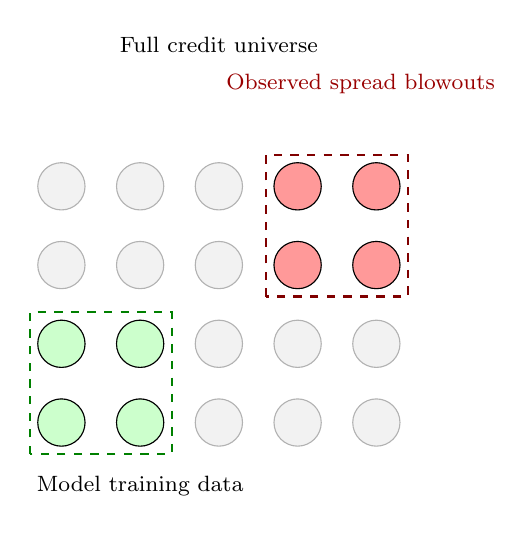
\begin{tikzpicture}[
      model/.style={circle, draw=black, fill=green!20, minimum size=0.6cm},
      blowout/.style={circle, draw=black, fill=red!40, minimum size=0.6cm},
      neutral/.style={circle, draw=black!30, fill=gray!10, minimum size=0.6cm},
      every node/.style={font=\scriptsize}
  ]
  
  % Credit universe grid (5x4)
  \foreach \x in {0,1,2,3,4} {
      \foreach \y in {0,1,2,3} {
          \node[neutral] (n\x\y) at (\x, \y) {};
      }
  }
  
  % Model training region (bottom-left 2x2)
  \foreach \x in {0,1} {
      \foreach \y in {0,1} {
          \node[model] at (\x, \y) {};
      }
  }
  
  % Blowout region (top-right 2x2)
  \foreach \x in {3,4} {
      \foreach \y in {2,3} {
          \node[blowout] at (\x, \y) {};
      }
  }
  
  % Labels
  \node[align=left, font=\footnotesize] at (1, -0.8) {Model training data};
  \node[align=left, font=\footnotesize, text=red!60!black] at (3.8, 4.3) {Observed spread blowouts};
  \node[align=left, font=\footnotesize] at (2, 4.8) {Full credit universe};
  
  \draw[dashed, thick, green!50!black] (-0.4, -0.4) rectangle (1.4, 1.4);
  \draw[dashed, thick, red!50!black] (2.6, 1.6) rectangle (4.4, 3.4);
  
  \end{tikzpicture}
  \caption{Spread Blowout Occurred Outside Model Coverage: The model was trained on credit names in calm regimes (green), but the shock hit an unmodeled set of issuers (red).}
\END{FIGURE}

\MEDSKIP

The AI never flagged this because it had learned from historical data that IG bonds and oil weren’t highly correlated.  
It assumed the CDS short would \textit{offset} the oil exposure.

Instead, both positions bled simultaneously.

\medskip

\begin{figure}[H]
  \centering
  \resizebox{\textwidth}{!}{%
  \begin{tikzpicture}[
    node distance=1.2cm and 2.2cm,
    every node/.style={font=\small},
    box/.style={draw, rounded corners, minimum width=3.8cm, minimum height=1.2cm, align=center, fill=gray!10},
    arrow/.style={->, thick}
  ]
  
  % Top layer (assumptions)
  \node[box] (data) {Narrow Training Data\\(Low-volatility, stable regime)};
  \node[box, right=of data] (assumption) {Learned Historical\\Decorrelation};
  \node[box, right=of assumption] (blindspot) {No Calibration for\\Joint Stress Events};
  
  % Middle layer (stress response)
  \node[box, below=2cm of blindspot] (shock) {Oil Collapse \& CDS Spread Blowout\\Ignored as Uncorrelated};
  \node[box, left=of shock] (margin) {Margin Calls Trigger Forced Selling};
  \node[box, left=of margin] (amplify) {Selling Widens Spreads\\Triggers More Margin Calls};
  
  % Bottom layer (outcomes)
  \node[box, below=2cm of margin] (late) {AI Issues Alert\\After 89\% Liquidity Is Gone};
  \node[box, right=of late, fill=red!20] (result) {\textbf{Catastrophic Losses}\\Portfolio -47\%};
  
  % Arrows (top layer)
  \draw[arrow] (data) -- (assumption);
  \draw[arrow] (assumption) -- (blindspot);
  
  % Arrows (top → middle)
  \draw[arrow] (blindspot.south) -- (shock.north);
  \draw[arrow] (shock) -- (margin);
  \draw[arrow] (margin) -- (amplify);
  
  % Arrows (middle → bottom)
  \draw[arrow] (amplify.south) -- (late.north);
  \draw[arrow] (late) -- (result);
  
  \end{tikzpicture}
  }
  \caption{Three-stage breakdown: flawed assumptions, failure under stress, and financial collapse.}
\end{figure}
  
\medskip

\medskip

\begin{figure}[H]
  \centering
  \resizebox{\textwidth}{!}{%
  \begin{tikzpicture}[node distance=1.5cm and 3cm, every node/.style={font=\small}]
  
  % Nodes
  \node[draw, align=center, fill=gray!10] (trigger) {Macro Trigger:\\\textbf{120bps rate hike}\\\textbf{+ Oil flash crash}};
  \node[draw, below=of trigger, fill=gray!10, align=center] (plunge) {\textbf{Oil futures collapse}\\$\downarrow$14\% in 30 min};
  \node[draw, below=of plunge, fill=gray!10, align=center] (portfolio) {Arcadia Portfolio:\\\textbf{Long oil and}\\\textbf{Short IG via CDS}};
  \node[draw, below=of portfolio, fill=gray!10, align=center] (margincall) {\textbf{Trigger margin calls}\\on futures positions};
  \node[draw, below left=of margincall, fill=gray!10, align=center] (liqbonds) {\textbf{Sells}\\\textbf{investment-grade bonds}\\to raise cash};
  \node[draw, below right=of margincall, fill=gray!10, align=center] (cdsspread) {\textbf{IG bond spreads widen}\\$\Rightarrow$ CDS short loses value};
  
  \node[draw, below=of margincall, fill=gray!10, align=center] (variation) {\textbf{Variation margin calls}\\from credit counterparties};
  
  % Arrows
  \draw[->, thick] (trigger) -- (plunge);
  \draw[->, thick] (plunge) -- (portfolio);
  \draw[->, thick] (portfolio) -- (margincall);
  \draw[->, thick] (margincall) -- (liqbonds);
  \draw[->, thick] (margincall) -- (cdsspread);
  \draw[->, thick] (cdsspread) -- (variation);
  
  % Feedback loop
  \draw[->, thick, dashed, bend left=30] (variation.north) to node[right, align=center] {\scriptsize More margin calls\\\scriptsize $\Rightarrow$ More selling} (margincall.south);
  
  \end{tikzpicture}
  }
  \caption{Cascade triggered by rate shock and oil crash: how feedback loops undid Arcadia.}
\end{figure}




He walked Hart through the core issues:

\begin{itemize}
  \item \textbf{The model was overfitting to recent market patterns} \\
  \\
  Imagine training a guard dog using only sounds from one specific neighborhood — it learns to bark only when it hears those familiar sounds.  
  The model was trained on a very specific kind of market behavior that happened after COVID — a period where the markets were calmer and often bounced back to normal. It learned those patterns really well... but only those. That made it fragile when things changed even slightly, like a dog that freezes when it hears a new noise.

  \item \textbf{There was no external validation} \\
  \\
  It’s like designing a car that drives well on a test track but never trying it on hills, in the rain, or in traffic.  
  The model was never tested on different types of markets — such as fast crashes, slow downturns, or unexpected shocks. Without that kind of testing, there's no way to know if the model works outside its comfort zone.

  \item \textbf{The training data was too narrow} \\
  \\
  Picture trying to predict national election results using surveys from only one small town.  
  The model only saw market data from limited, local regions. So it didn’t learn how national or global trends — like a crisis in Europe or a U.S. interest rate hike — might ripple across different areas.

  \item \textbf{It was never stress-tested across economic cycles} \\
  \\
  Like building a bridge and only testing it on sunny days — never during storms, floods, or heavy traffic.  
  The model only experienced one kind of economic environment: low interest rates, stable markets, and lots of money flowing around. It had no exposure to downturns, recessions, or high inflation periods. So we don’t know how it would react when things get rough.

  \item \textbf{It wasn’t calibrated for outliers} \\
  \\
  Imagine planning your day based on weather forecasts, but your app doesn’t even consider the chance of tornadoes or earthquakes.  
  The model didn’t prepare for rare but catastrophic events — like sudden policy changes, huge bankruptcies, or natural disasters. These events may be rare, but when they happen, they can break systems that weren’t built with those possibilities in mind.
\end{itemize}


\medskip

\begin{figure}[H]
  \centering
  \begin{tikzpicture}
  \matrix[matrix of nodes,
          nodes={minimum width=1.8cm, minimum height=1cm, text centered, draw=black},
          row sep=-\pgflinewidth, column sep=-\pgflinewidth,
          column 1/.style={nodes={text width=2.5cm, align=right}},
          column 2/.style={nodes={fill=red!10}},
          column 3/.style={nodes={fill=red!20}},
          column 4/.style={nodes={fill=red!40}},
          column 5/.style={nodes={fill=red!70}},
          column 6/.style={nodes={fill=red!90, text=white}},
          ] 
  {
  \textbf{Market Regime} & \textbf{2013} & \textbf{2015} & \textbf{2018} & \textbf{2020} & \textbf{2022} \\
  Low Volatility         &  ✓           &  ✓✓          &  ✓✓✓         &  ✓✓✓✓        &  ✓✓✓✓✓       \\
  Mild Correction        &              &   ✓          &   ✓✓         &   ✓✓         &   ✓✓         \\
  Policy Shock           &              &              &              &   ✓          &   ✓          \\
  Liquidity Crisis       &              &              &              &   ✗          &   ✗          \\
  Regime Shift           &              &              &              &              &   ✗          \\
  };
  
  % Caption
  \end{tikzpicture}
  \caption{Model Training Bias: Aurora AI was trained mostly on low-volatility environments, with sparse or no exposure to structural shocks or liquidity breakdowns.}
\end{figure}
 
\medskip